\subsection{CIB内電源回路}



通信用マイコンであるRXCOBC,TXCOBCはミッション開始から終了まで非常時を除きすべての期間で起動している必要がある.EPSから電源供給されるコンポーネントの一括ON/OFFを可能にするためにこれらの電源系はEPS基板とは別に新たに設け,EPS電源が入っていない状態においても衛星として最低限の役割が機能するように設計した.RXCOBC,TXCOBCの電源であるCIB内の3.3 V系には一般的に効率の良いスイッチングレギュレータではなく信頼性の高いリニアレギュレータを使用した.さらにレギュレータが1つ動作しなかった場合に備えて二つのレギュレータを並列で繋いだ(図\ref{fig3_1_3V3}).一般にリニアレギュレータの並列はORダイオードを用いて行われる\cite{reg_um}.

\begin{figure}[htbp]
	\begin{center}
		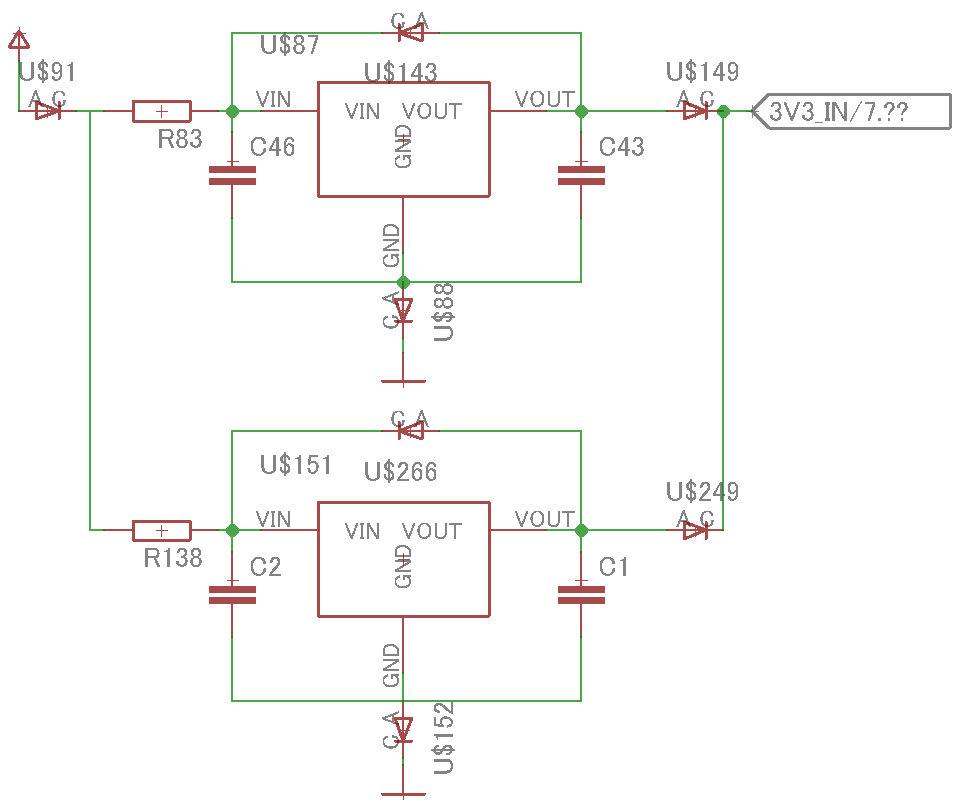
\includegraphics[width=0.6\linewidth]{./03/fig/3V3.png}
		\caption{Paralleling Linear Regulators Schematic}
		\label{fig3_1_3V3}
	\end{center}
\end{figure}

UHF/VHF無線機はEPSからの供給をメインとし,EPS非起動時にも通信が行えるように5VをCIB内でリニアレギュレータを用いて生成できるようにした.

さらに5.8GHz送信を行う際の突入電流によりEPSの過電流保護機能が働き,他の機器への影響がでてしまうため昇圧スイッチング・レギュレータを用いて12V系も新たにCIB上に設計した.さらにレギュレータの故障による過電流防止のために,
ICを設けた.また放射線試験によるICの放射線耐性を入念に確認した.

